\section{¿Qué tenemos?}
\subsection{Paso de mensajes bajo IPv4}
\begin{frame}
  \frametitle{Mensajes desde VM al Labcomp}
  \begin{columns}[t]
    \column{0.5\textwidth}
    	\begin{figure}
		\centering
		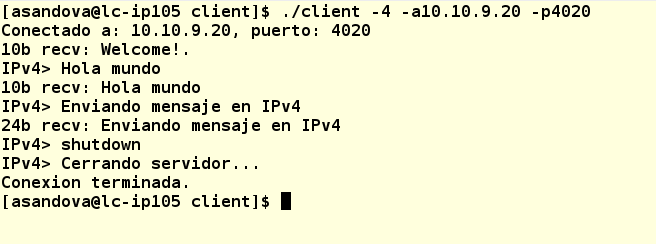
\includegraphics[width=150px]{img/ipv4-client.png}
	\end{figure}
    \column{0.5\textwidth}
    	\begin{figure}
		\centering
		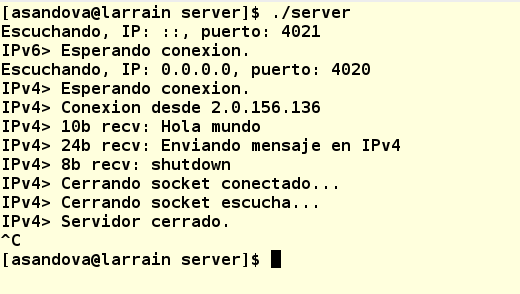
\includegraphics[width=150px]{img/ipv4-server.png}
	\end{figure}
  \end{columns}
\end{frame}

\subsection{Paso de mensajes bajo IPv6}
\begin{frame}
  \frametitle{Mensajes entre dos máquinas del Labcomp}
  \begin{columns}[t]
    \column{0.5\textwidth}
    	\begin{figure}
		\centering
		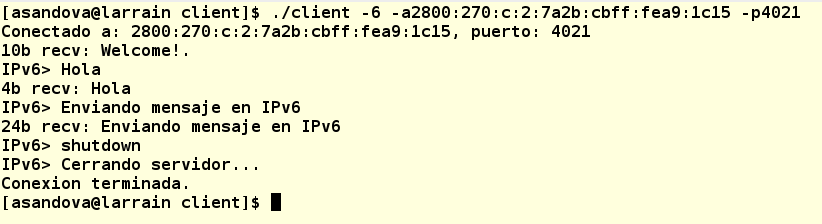
\includegraphics[width=150px]{img/ipv6-client.png}
	\end{figure}
    \column{0.5\textwidth}
    	\begin{figure}
		\centering
		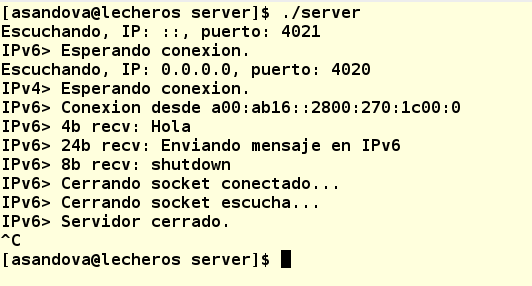
\includegraphics[width=150px]{img/ipv6-server.png}
	\end{figure}
   \end{columns}
\end{frame}

\subsection{Documentación}
\begin{frame}
	\centering
	Documentación (Ver Sitio del Proyecto).
\end{frame}


\subsection{Problemas}
\begin{frame}
  \frametitle{Direcciones IPv6}
   \begin{columns}[t]
    \column{0.5\textwidth}
    	\begin{figure}
		\centering
		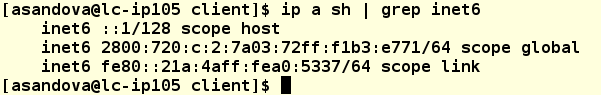
\includegraphics[width=150px]{img/ipv6-VMconf.png}
	\end{figure}
    \column{0.5\textwidth}
    	\begin{figure}
		\centering
		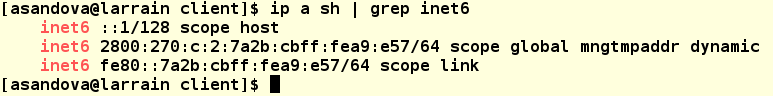
\includegraphics[width=170px]{img/ipv6-LabConf.png}
	\end{figure}
    \end{columns}
\end{frame}

\begin{frame}
  \frametitle{¿Por qué no Labcomp-VM?}
  \begin{columns}[t]
    \column{0.5\textwidth}
    	\begin{figure}
		\centering
		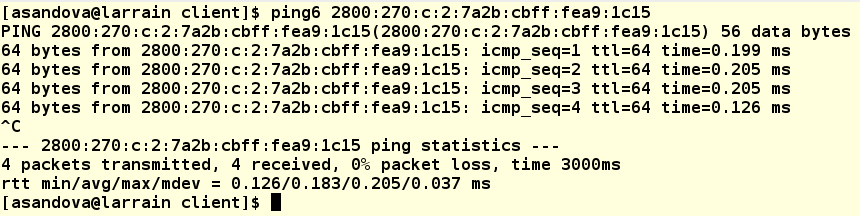
\includegraphics[width=150px]{img/ping6-lab-lab.png}
	\end{figure}
    \column{0.5\textwidth}
    	\begin{figure}
		\centering
		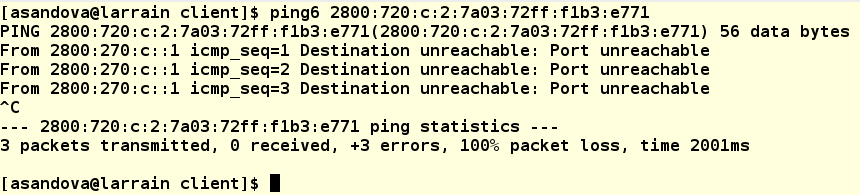
\includegraphics[width=150px]{img/ping6-lab-vm.png}
	\end{figure}
  	\begin{figure}
		\centering
		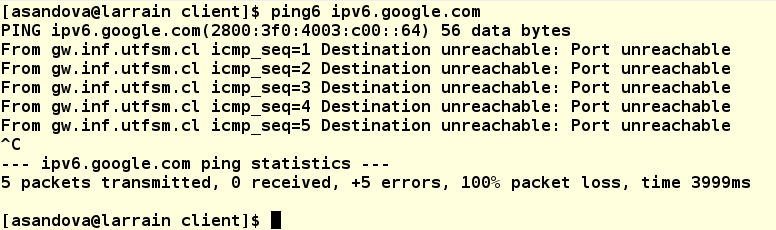
\includegraphics[width=150px]{img/ping6-lab-gv6.png}
	\end{figure}
  \end{columns}
\end{frame}





